
%(BEGIN_QUESTION)
% Copyright 2014, Tony R. Kuphaldt, released under the Creative Commons Attribution License (v 1.0)
% This means you may do almost anything with this work of mine, so long as you give me proper credit

Determine the total current and all voltage drops in this circuit, stating your answers the way a multimeter would register them:

$$\includegraphics[width=15.5cm]{i01070x01.eps}$$

\goodbreak

\item{} $C_1 = 125 \hbox{ pF}$
\item{} $C_2 = 71 \hbox{ pF}$
\item{} $R_1 = 6.8 \hbox{ k}\Omega$
\item{} $R_2 = 1.2 \hbox{ k}\Omega$
\item{} $V_{supply} = 20 \hbox{ V RMS}$
\item{} $f_{supply} = 950 \hbox{ kHz}$

\vskip 10pt

Also, calculate the phase angle ($\theta$) between voltage and current in this circuit, and explain where and how you would connect an oscilloscope to measure that phase shift.

\underbar{file i01070}
%(END_QUESTION)





%(BEGIN_ANSWER)

\item{} $I_{total} = 2.269 \hbox{ mA}$
\item{} $V_{C1} = 3.041 \hbox{ V}$
\item{} $V_{C2} = 5.354 \hbox{ V}$
\item{} $V_{R1} = 15.43 \hbox{ V}$
\item{} $V_{R2} = 2.723 \hbox{ V}$
\item{} $\theta = -24.82^o$ (voltage lagging current)
\end{itemize}

I suggest using a dual-trace oscilloscope to measure total voltage (across the supply terminals) and voltage drop across resistor $R_2$.  Theoretically, measuring the voltage dropped by either resistor would be fine, but $R_2$ works better for practical reasons (oscilloscope input lead grounding).  Phase shift then could be measured either in the time domain or by a Lissajous figure analysis.

%(END_ANSWER)





%(BEGIN_NOTES)

Some students many wonder what type of numerical result best corresponds to a multimeter's readings, if they do their calculations using complex numbers (``do I use polar or rectangular form, and if rectangular do I use the real or the imaginary part?'').  The answers given for this question should clarify that point.

It is very important that students know how to apply this knowledge of AC circuit analysis to real-world situations.  Asking students to determine how they would connect an oscilloscope to the circuit to measure $\theta$ is an exercise in developing their abstraction abilities between calculations and actual circuit scenarios.

It is noteworthy that the low capacitances shown here approach parasitic capacitances between circuit board traces.  In other words, whoever designs a circuit to operate at 950 kHz cannot simply place components at will on the board, but must consider the traces themselves to be circuit elements (both capacitive and inductive in nature!).  The calculations used to obtain the given answers, of course, assume ideal conditions where the PC board is not considered to possess capacitance or inductance.

\vskip 10pt

Students often have difficulty formulating a method of solution: determining what steps to take to get from the given conditions to a final answer.  While it is helpful at first for you (the instructor) to show them, it is bad for you to show them too often, lest they stop thinking for themselves and merely follow your lead.  A teaching technique I have found very helpful is to have students come up to the board (alone or in teams) in front of class to write their problem-solving strategies for all the others to see.  They don't have to actually do the math, but rather outline the steps they would take, in the order they would take them.  The following is a sample of a written problem-solving strategy for analyzing a series resistive-reactive AC circuit:

\vskip 10pt

\goodbreak

{\bf Step 1:} Calculate all reactances ($X$).

{\bf Step 2:} Draw an impedance triangle ($Z$ ; $R$ ; $X$), solving for $Z$

{\bf Step 3:} Calculate circuit current using Ohm's Law: $I = {V \over Z}$

{\bf Step 4:} Calculate series voltage drops using Ohm's Law: $V = {I Z}$

{\bf Step 5:} Check work by drawing a voltage triangle ($V_{total}$ ; $V_1$ ; $V_2$), solving for $V_{total}$

\vskip 10pt

By having students outline their problem-solving strategies, everyone gets an opportunity to see multiple methods of solution, and you (the instructor) get to see how (and if!) your students are thinking.  An especially good point to emphasize in these ``open thinking'' activities is how to check your work to see if any mistakes were made.

%INDEX% Electronics review: AC reactance and impedance

%(END_NOTES)


